\chapter{数学公式排版}

% =========================================================
\section{行内公式与块级公式}
LaTeX 强大的数学排版功能是其最受欢迎的特性之一。在数学模式中，公式可以分为两大类：行内公式 和 块级公式。
\subsection{行内公式}
行内公式用于在正文中嵌入较短的数学表达式，通常用来书写变量、简单公式或符号。常用的写法有两种：
\begin{itemize}
	\item [美元符号法：]使用一对美元符号 \$...\$ 将数学表达式包裹起来。
	
	\item [圆括号法：]使用 \begin{lstlisting}
		\(...\)
	\end{lstlisting}同样可以达到行内公式的效果，通常这种方式更具可读性。
\end{itemize}
在行内公式中，LaTeX 会自动调整字体和间距，使得数学表达式与周围文本保持协调。但如果公式过长或复杂，则建议使用块级公式，以避免影响正文排版。

\subsection{块级公式}
块级公式用于单独展示较长或较重要的数学表达式，通常居中显示，并且可以自动编号（或取消编号）。常见的写法有以下几种：
\begin{enumerate}
	\item 使用\begin{lstlisting}
		\[。。。\]
	\end{lstlisting}这是最简单的块级公式写法，不会产生公式编号，适用于无需引用的公式。
	
	\item 使用 \texttt{equation} 环境
	该环境适用于需要编号的公式，方便后续引用。使用前记得引入 \texttt{amsmath} 包。
	\begin{lstlisting}
\begin{equation}
	\label{eq:quadratic}
	ax^2+bx+c=0
\end{equation}
	\end{lstlisting}
	可以在文中通过 \begin{lstlisting}
		\eqref{eq:quadratic}
	\end{lstlisting} 来引用该公式。
	\item 使用 align 环境
	对于多个相关联的公式或者需要对齐等号的情况，align 环境非常实用。同样需要加载 amsmath 包。
\end{enumerate}
% =========================================================
\section{数学符号与运算符}
见本章最后。
\begin{lstlisting}
% 行内公式中使用希腊字母
设 $\alpha, \beta, \gamma$ 为角度，而 $\Gamma(n)$ 表示伽马函数。
\end{lstlisting}
\subsection{上下标}
上下标是数学表达式中常见的元素，LaTeX 提供了简单的语法来实现它们。使用 \texttt{\^} 来表示上标，使用 \texttt{\_} 来表示下标。例如：
\begin{lstlisting}
% 上标和下标示例
设 $x_i$ 表示第 $i$ 个数据点，而 $y^2$ 表示 $y$ 的平方。
\end{lstlisting}

\subsection{分数与根号}
分数可以使用 \texttt{\textbackslash frac} 命令来表示，语法为 \texttt{\textbackslash frac{分子}{分母}}。例如：
\begin{lstlisting}
% 分数示例
设 $\frac{a}{b}$ 表示 $a$ 除以 $b$。
\end{lstlisting}
\begin{mybox}
	连分数可以使用 \texttt{\textbackslash cfrac} 命令来表示，语法为 \texttt{\textbackslash cfrac{分子}{分母}}。例如：
\begin{lstlisting}
% 连分数示例
设 $\cfrac{1}{2 + \cfrac{1}{3}}$ 表示一个连分数。
\end{lstlisting}
或者直接分数嵌套使用。
\end{mybox}
根号可以使用 \texttt{\textbackslash sqrt} 命令来表示，语法为 \texttt{\textbackslash sqrt{被开方数}}。例如：
\begin{lstlisting}
% 根号示例
设 $\sqrt{x}$ 表示 $x$ 的平方根。
\end{lstlisting}


% =========================================================


\section{矩阵、多行方程组与编号控制}
下面是一个带编号的多行对齐方程组（使用 \texttt{\&} 对齐等号） ：
\begin{equation}
\begin{aligned}
    (a+b)^2 &= a^2 + 2ab + b^2 \\
    (a-b)^2 &= a^2 - 2ab + b^2
\end{aligned}
\end{equation}

如果是排版方括号矩阵，可以使用 \texttt{bmatrix} 环境 ：
\begin{equation}
    A = \begin{bmatrix}
        a_{11} & a_{12} \\
        a_{21} & a_{22}
    \end{bmatrix}
\end{equation}

\bigskip
\begin{lstlisting}[language={[LaTeX]TeX}, caption={矩阵排版源代码参考}]
\begin{bmatrix}
    a_{11} & a_{12} \\
    a_{21} & a_{22}
\end{bmatrix}
\end{lstlisting}

如果是排版圆括号矩阵，可以使用 \texttt{pmatrix} 环境 ：
\begin{equation}
	B = \begin{pmatrix}
		b_{11} & b_{12} \\
		b_{21} & b_{22}
	\end{pmatrix}
\end{equation}

还有范数符号（双竖线），使用 \texttt{Vmatrix} 来表示：
\begin{lstlisting}
\lVert v \rVert = \begin{Vmatrix}
x \\
y \\
z
\end{Vmatrix}
\end{lstlisting}

\section{妙招}
依旧如果我们不适应这种直接敲公式的方法，我还有小妙招！
https://www.latexlive.com/home
这个网站可以把公式转换为tex，或者Mathtype（Word里面的一个插件，小顾你以后一定会用）中直接复制出来，就是LaTeX格式，其实很方便。


\section{符号大全}
这是我常用的一个符号查找的表。是我用Markdown的时候用的。Markdown和\LaTeX 的符号是一样的。


% 每个图片独立为一个 figure 环境
% [htb!] 建议 LaTeX 优先放在此处，t 代表页顶，b 代表页底，! 代表加强建议

\begin{figure}[htb!]
	\centering
	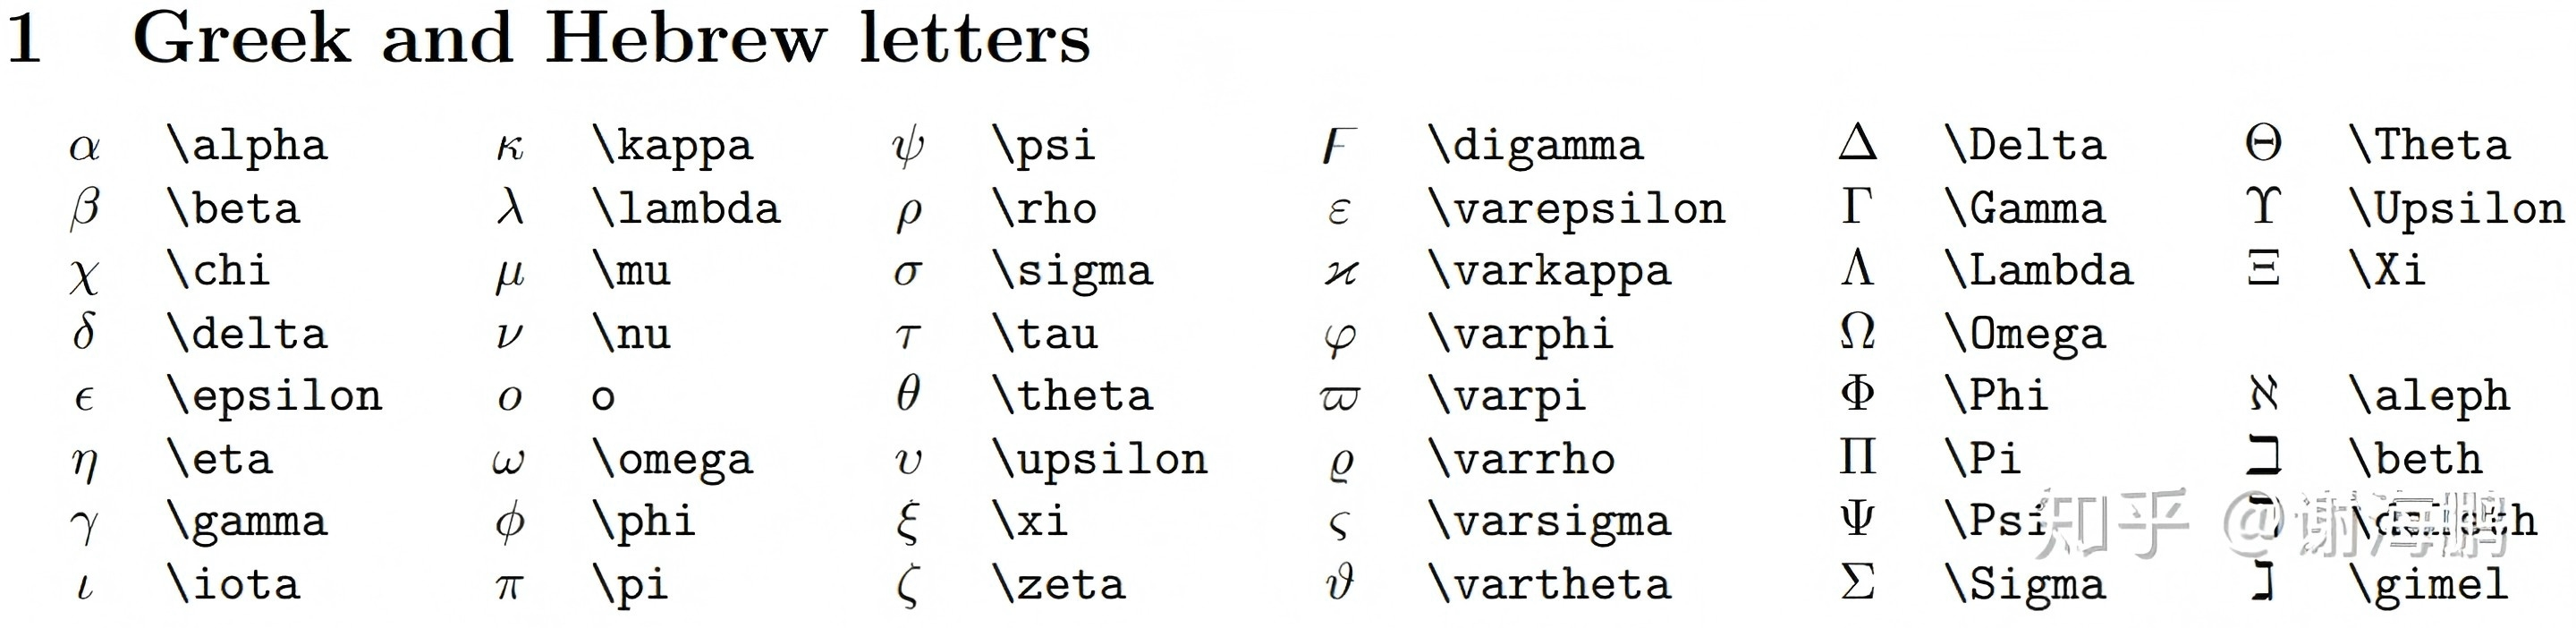
\includegraphics[width=1.0\textwidth]{Figure/1.jpg}
	\caption{希腊字母和希伯来字母表}
\end{figure}

\begin{figure}[htb!]
	\centering
	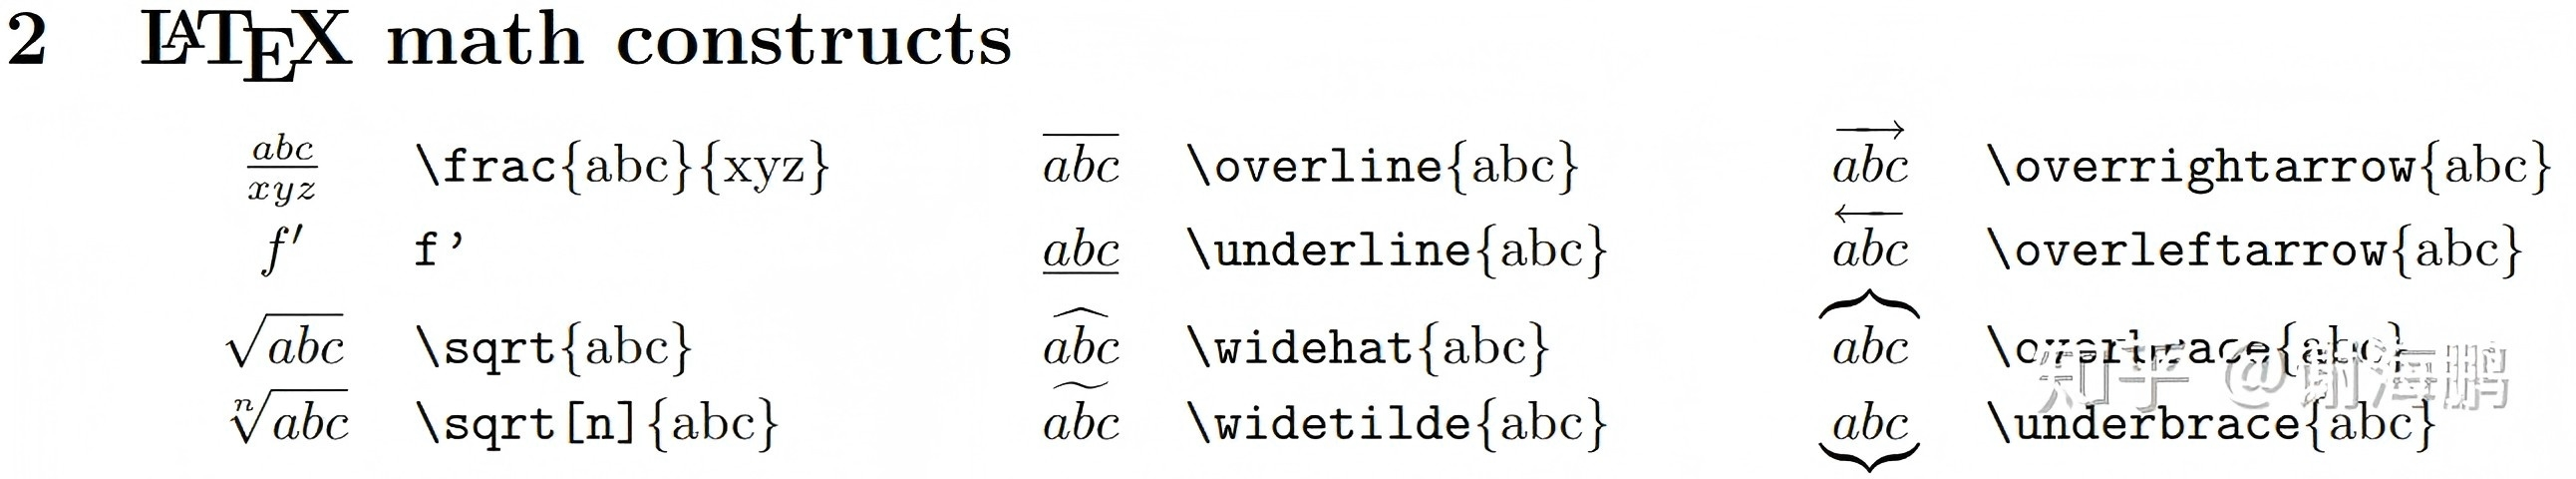
\includegraphics[width=1.0\textwidth]{Figure/2.jpg}
	\caption{LaTeX 数学表达式}
\end{figure}

\begin{figure}[htb!]
	\centering
	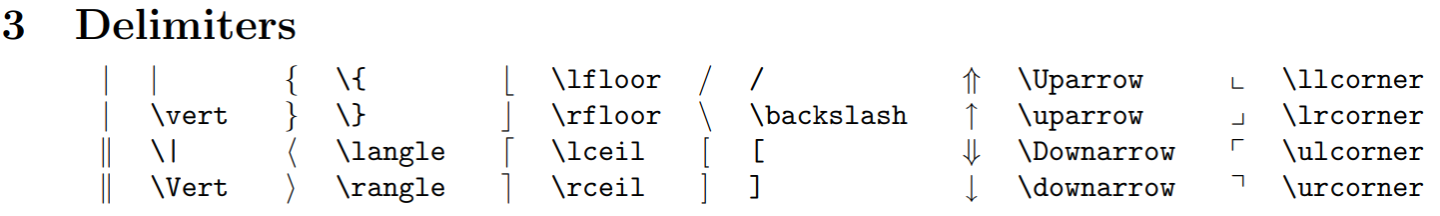
\includegraphics[width=1.0\textwidth]{Figure/3.png}
	\caption{分隔符和箭头符号}
\end{figure}

\begin{figure}[htb!]
	\centering
	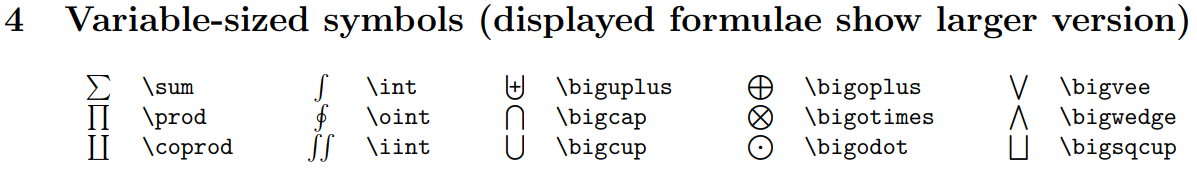
\includegraphics[width=1.0\textwidth]{Figure/4.png}
	\caption{可变长度符号}
\end{figure}

\begin{figure}[htb!]
	\centering
	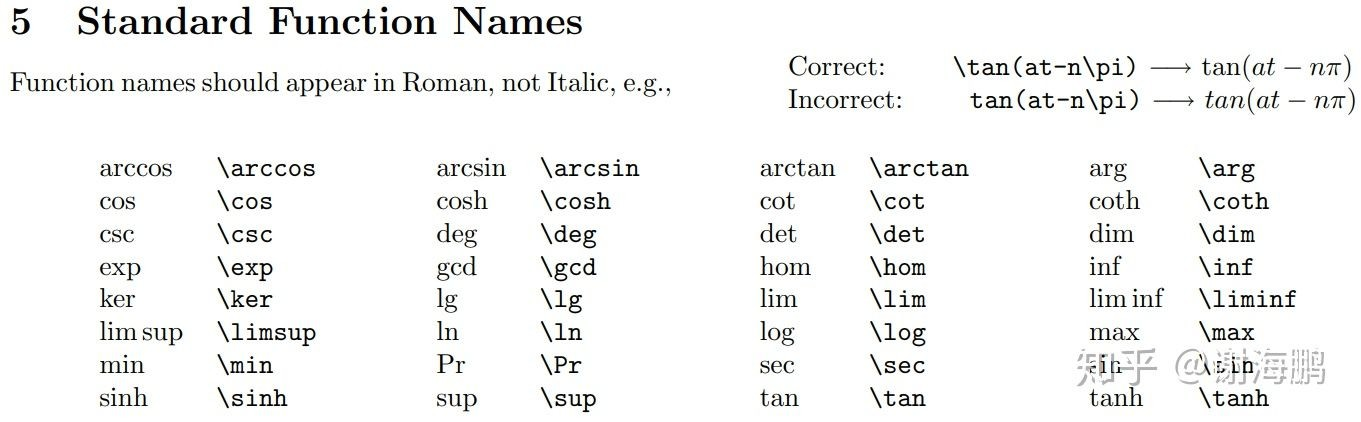
\includegraphics[width=1.0\textwidth]{Figure/5.jpg}
	\caption{标准函数名}
\end{figure}

\begin{figure}[htb!]
	\centering
	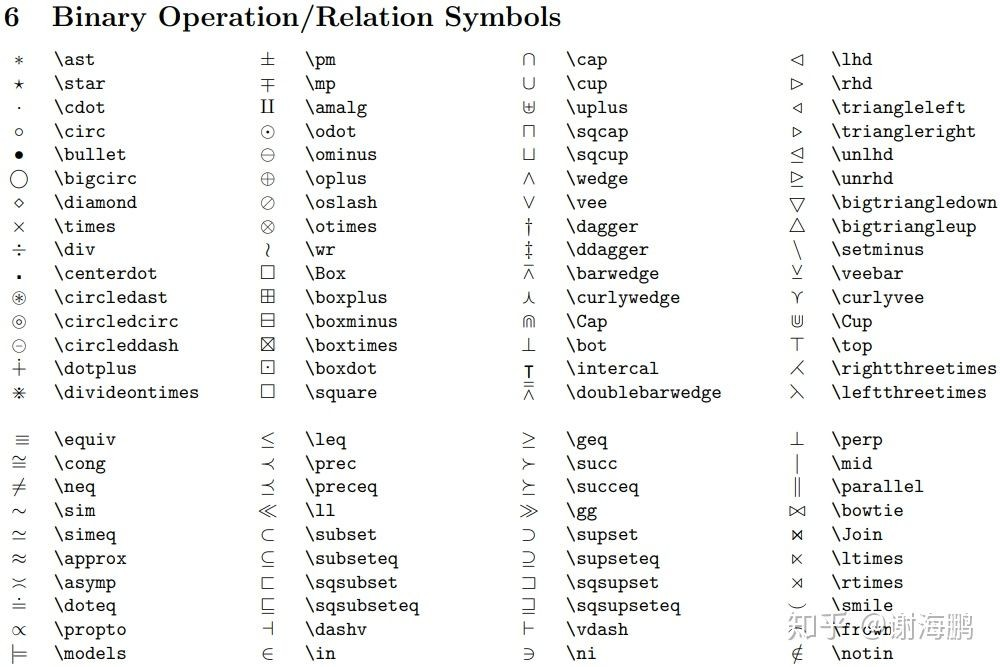
\includegraphics[width=1.0\textwidth]{Figure/6.jpg}
	\caption{二元运算符和关系运算符}
\end{figure}
\newpage
\begin{figure}
	\centering
	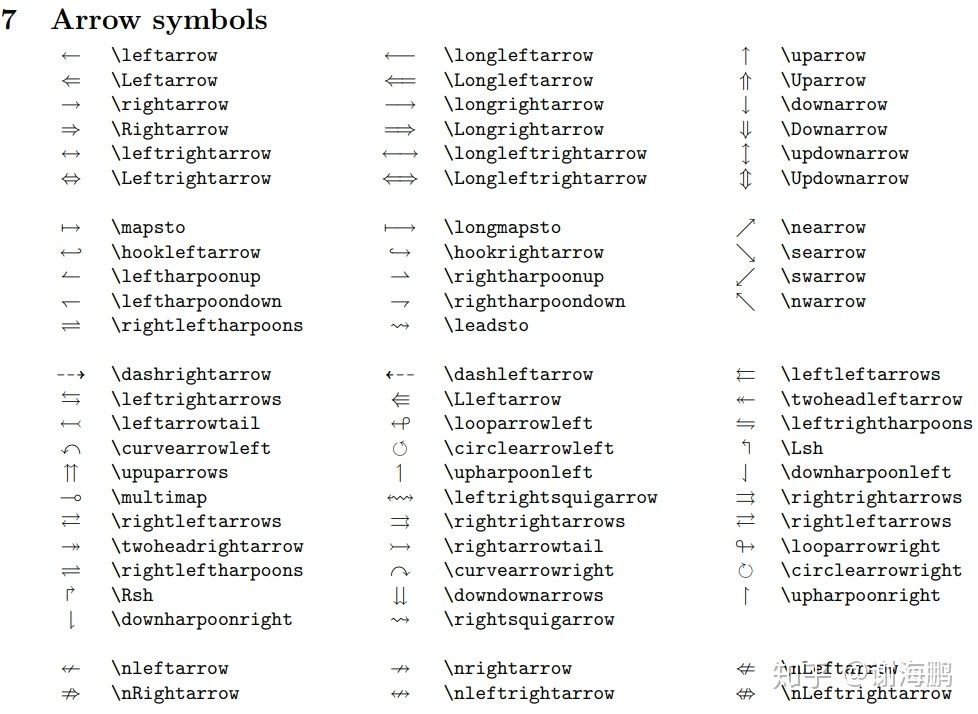
\includegraphics[width=1.0\textwidth]{Figure/7.jpg}
	\caption{箭头符号和其他符号}
\end{figure}

\begin{figure}
	\centering
	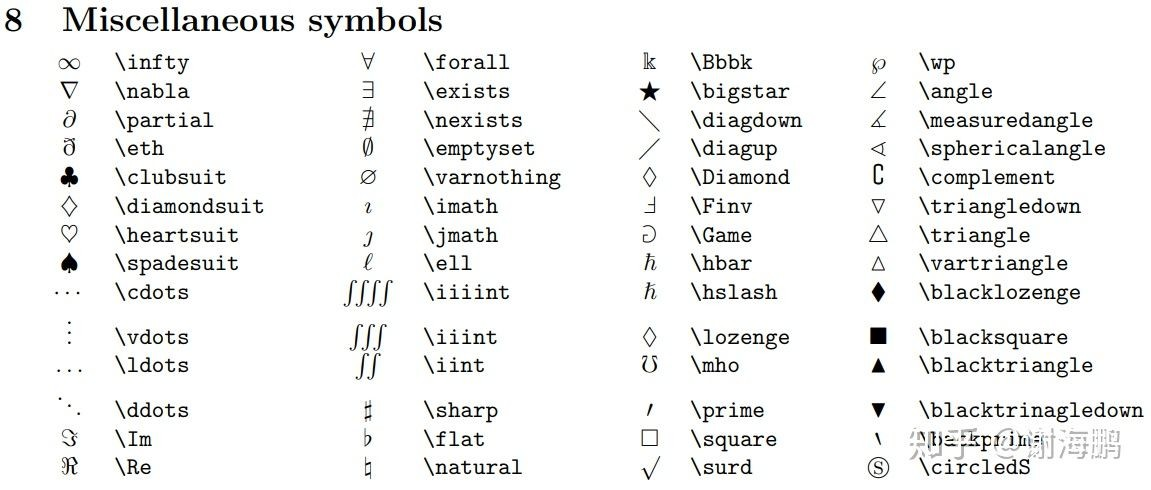
\includegraphics[width=1.0\textwidth]{Figure/8.jpg}
	\caption{杂项符号}
\end{figure}
当然Texshop本身就提供了一个快速插入符号的符号表。就在VSCode的侧边栏里。点击LaTeX Workshop的图标就可以看到符号表了。
% =========================================================